

\begin{mydef}

	Deux figures sont \kw{symétriques par rapport à un point $O$} si elles se superposent lorsqu'on effectue un demi-tour autour du point $O$. Le point $O$ est appelé \kw{centre de symétrie}.
	
\end{mydef}

\begin{myex}
	\begin{center}
		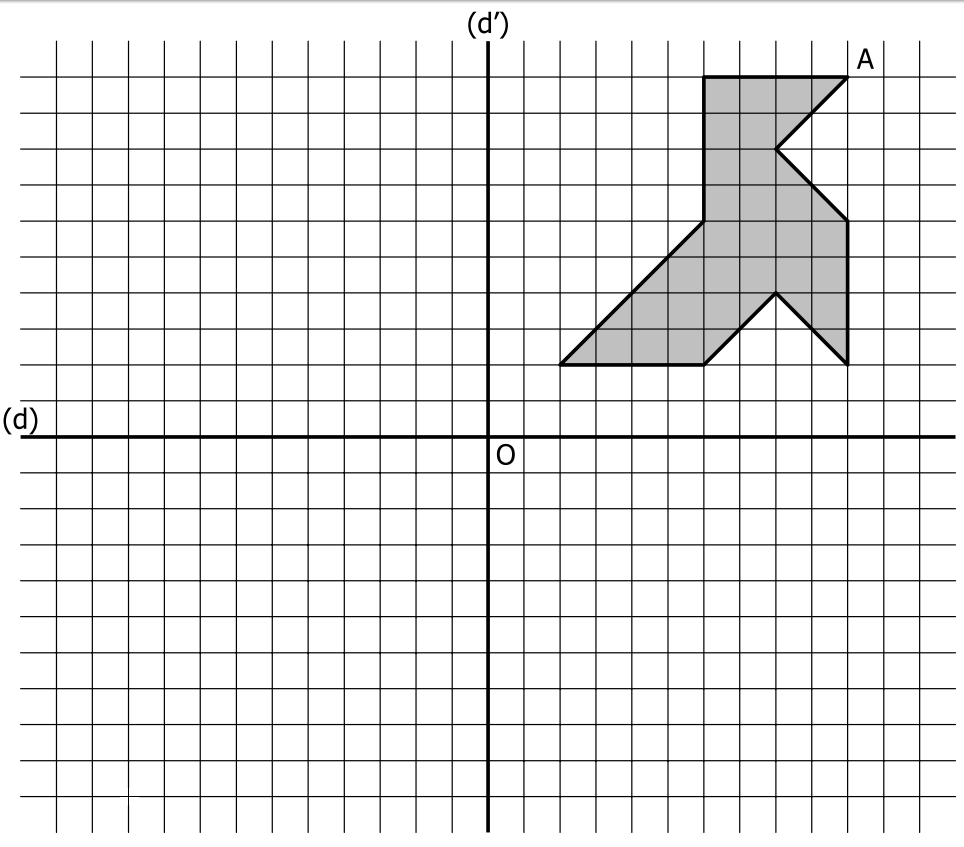
\includegraphics[scale=.75]{fig2}
	\end{center}
\end{myex}

